%----------------------------------------------------------
\def\notedate{2021.05.12}
\def\currentauthor{Ершов В. (РК6-72Б)}
%----------------------------------------------------------
\notestatement{rndhpcedt}{Описание текущего состояния проекта}

В данной заметке описаны все основные пользовательские сценарии web-ориентированного редактора графов на состояние от 2021.12.05. Для каждого сценария составлен следующий список:
\begin{itemize}
	\item Реализованные возможности сценария
	\item Сложности, возникшие при реализации сценария
	\item Будущий функционал, который расширит user expirience
\end{itemize}
Основые сценарии приложения:
\begin{itemize}
	\item Создание графа в приложении путем добавления вершин и ребер между ними
	\item Экспортирование графа в файл на языке описания графов aDOT
	\item Импортирование графа из файла на языке описания графов aDOT
\end{itemize}

\textbf{Добавление вершины}

Для доблавения вершины необходимо выбрать соответствующий пункт в меню, а затем кликнуть на холст.
После этого потребуется уточнить название вершины, после ввода названия вершины построение будет полностью завершено. Процесс построения вершины представлен на рисунке \ref{fig:vertex_create_1}.

\begin{figure}[h!]
\center{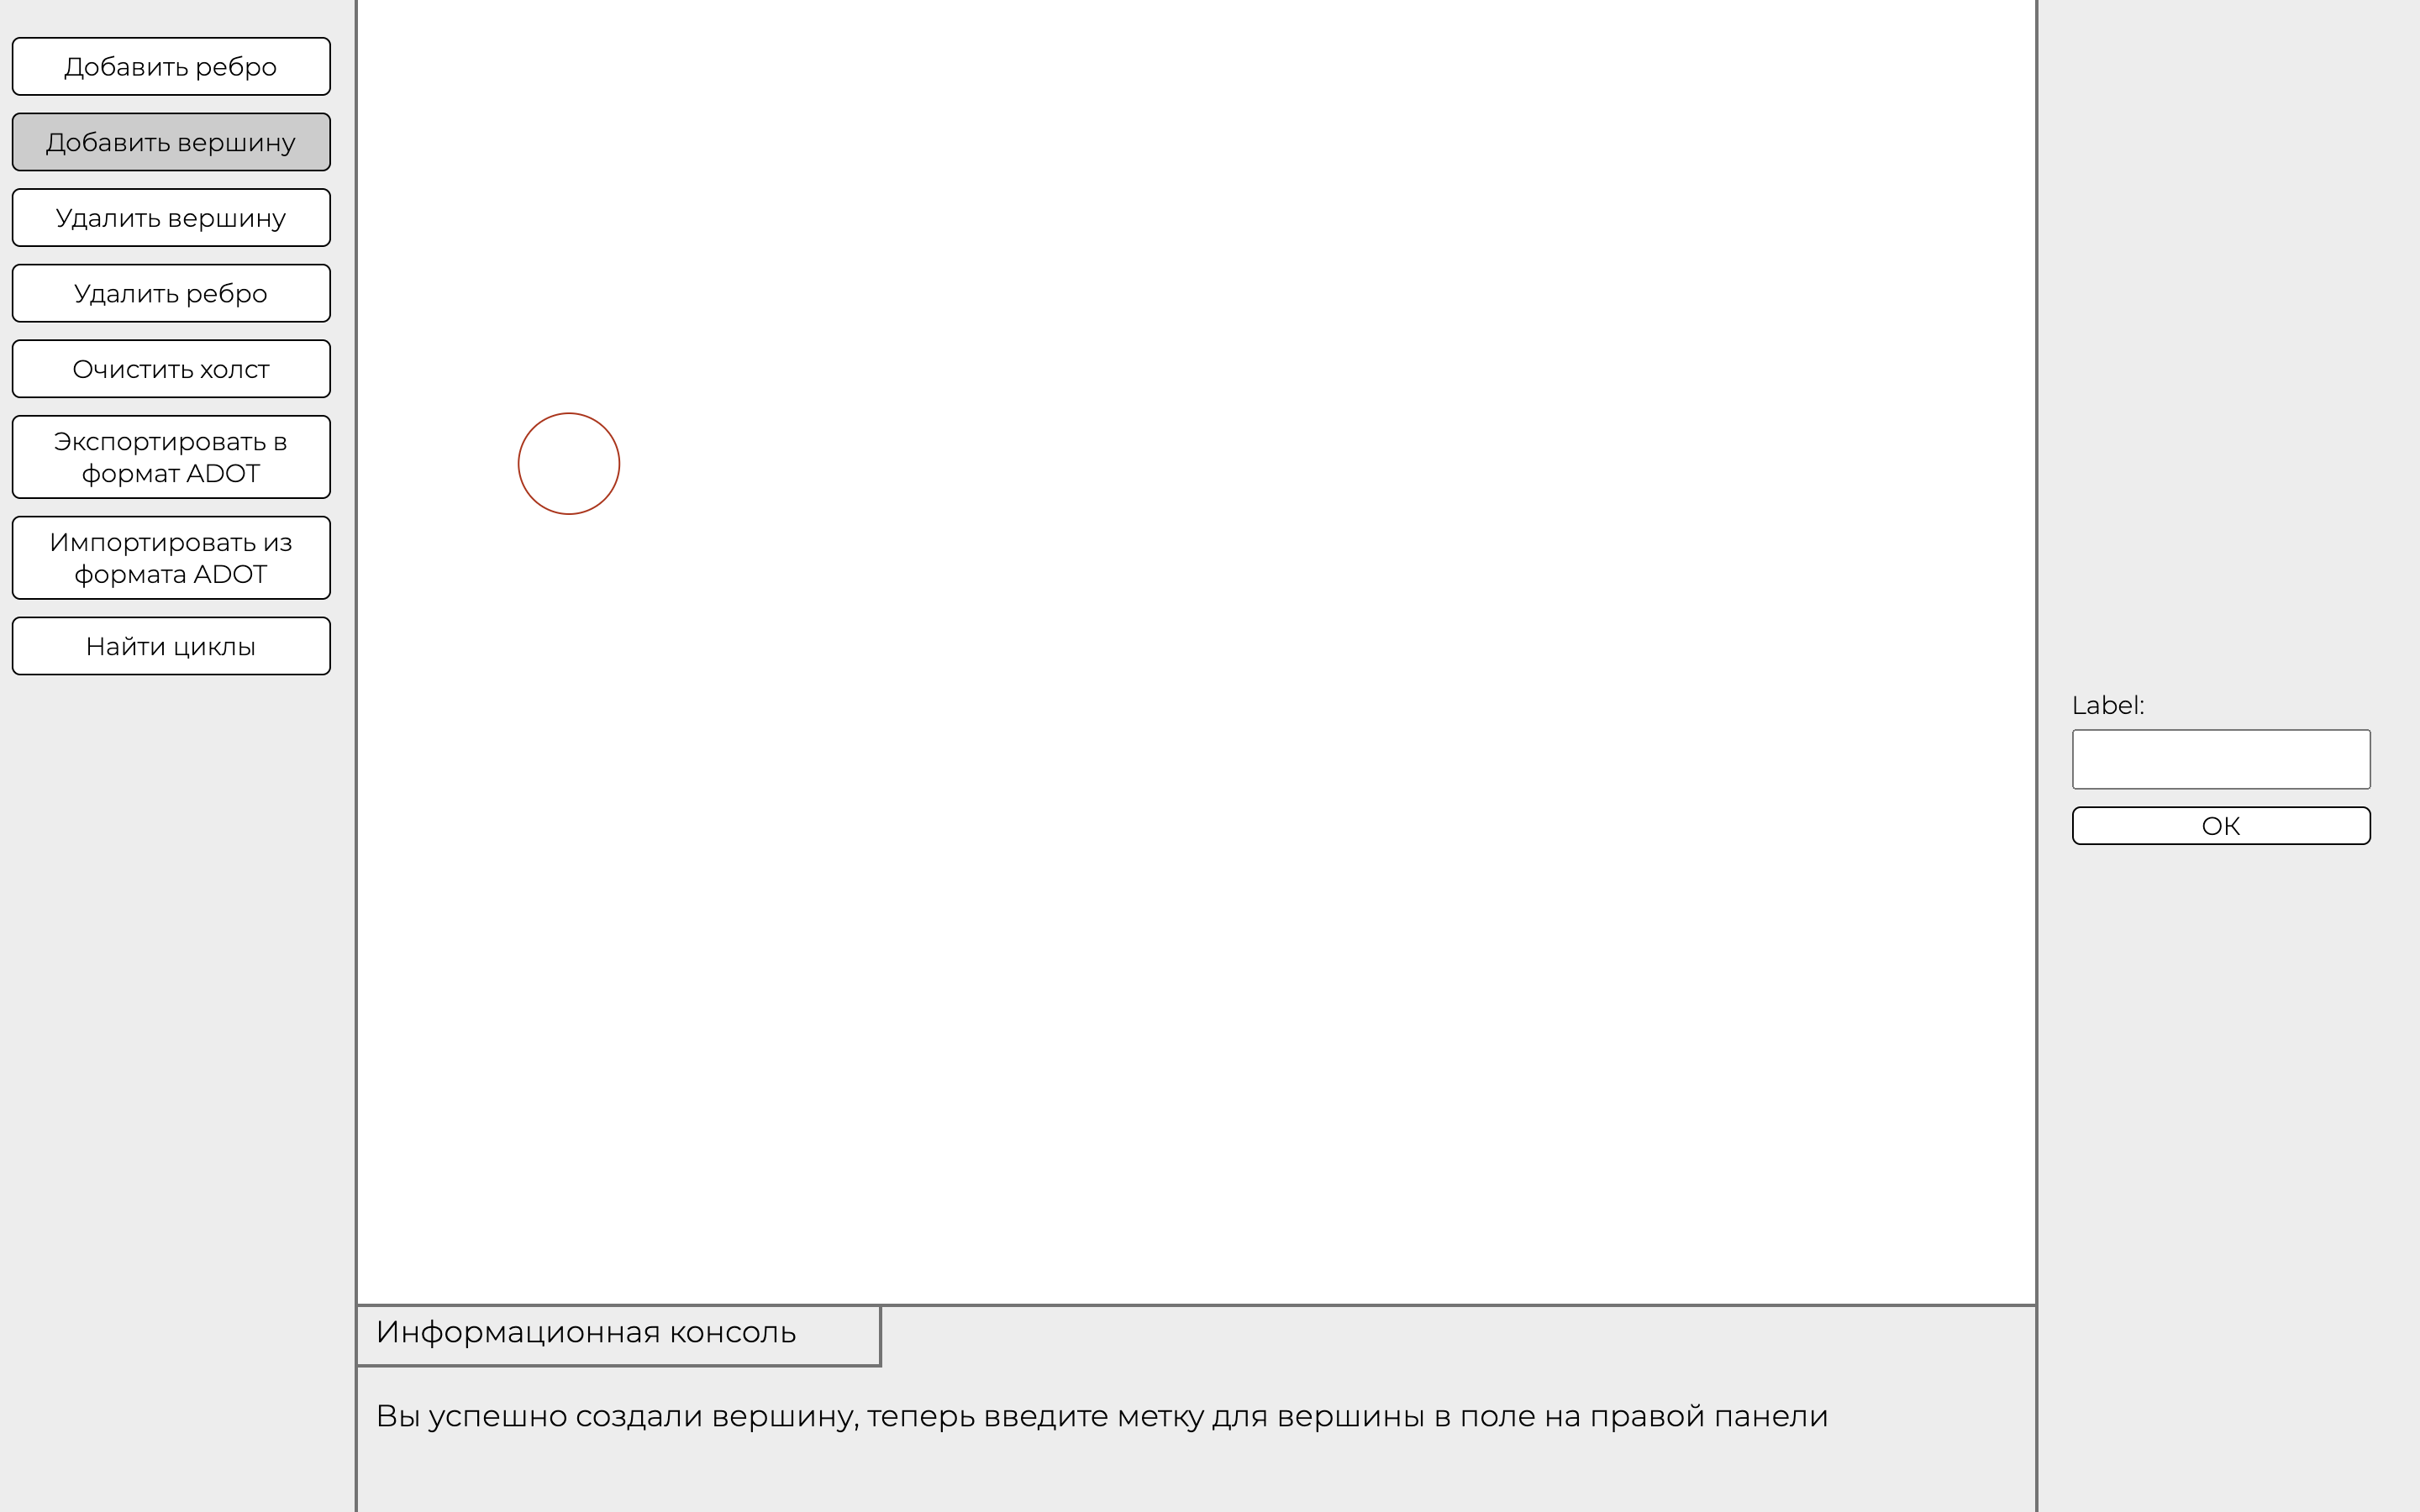
\includegraphics[width=0.9\linewidth]{ResearchNotes/images/vertex_create_1.png}}
\caption{Создание вершины}
\label{fig:vertex_create_1}
\end{figure}

Дополнительный функционал сценария:
\begin{itemize}
	\item Блокировка создания вершины если она находится в близости к другой вершине
	\item Блокировка создания названия вершины, если такое название присвоено существующей вершине
\end{itemize}

Сложности при реализации сценария:
\begin{itemize}
	\item Валидировать все необходимые параметры в процессе создания вершины: положение вершины, название вершины
	\item Выбор информации о вершине, которую нужно сохранить в оперативной памяти для дальнейшего использования в других сценариях
\end{itemize}

Будущее расширение функционала сценария:
\begin{itemize}
	\item Возможность изменить положение вершины в процессе ее создания. На данный момент вершина создается в месте клика на холст (в том случае если местоположение вершины валидно) и это местоположение уже никак нельзя изменить.
	\item Использование набора горячих клавиш для ускорения процесса создания вершины
	\item При  названия подсказать пользователю название вершины, в том случае если прошлые названия имеют инкрементирующийся для каждой вершины постфикс, например, уже созданы вершины $s_1, s_2$, при создании новой вершины в поле ввода названия система предложит пользователю название $s_3$.
\end{itemize}

\textbf{Добавление ребра}

Для добавления ребра необходимо поочередно выбрать две вершины, которые будут соединены ребром. Затем система потребует ввода предиката и функции, в том случае если введенный предикат или функция являются уникальнальными в рамках графа, то система потребует ввода информации о module и entry func. После этого построение ребра будет завершено. Процесс построения ребра представлен на рисунке \ref{fig:edge_create}.

\begin{figure}[h!]
\center{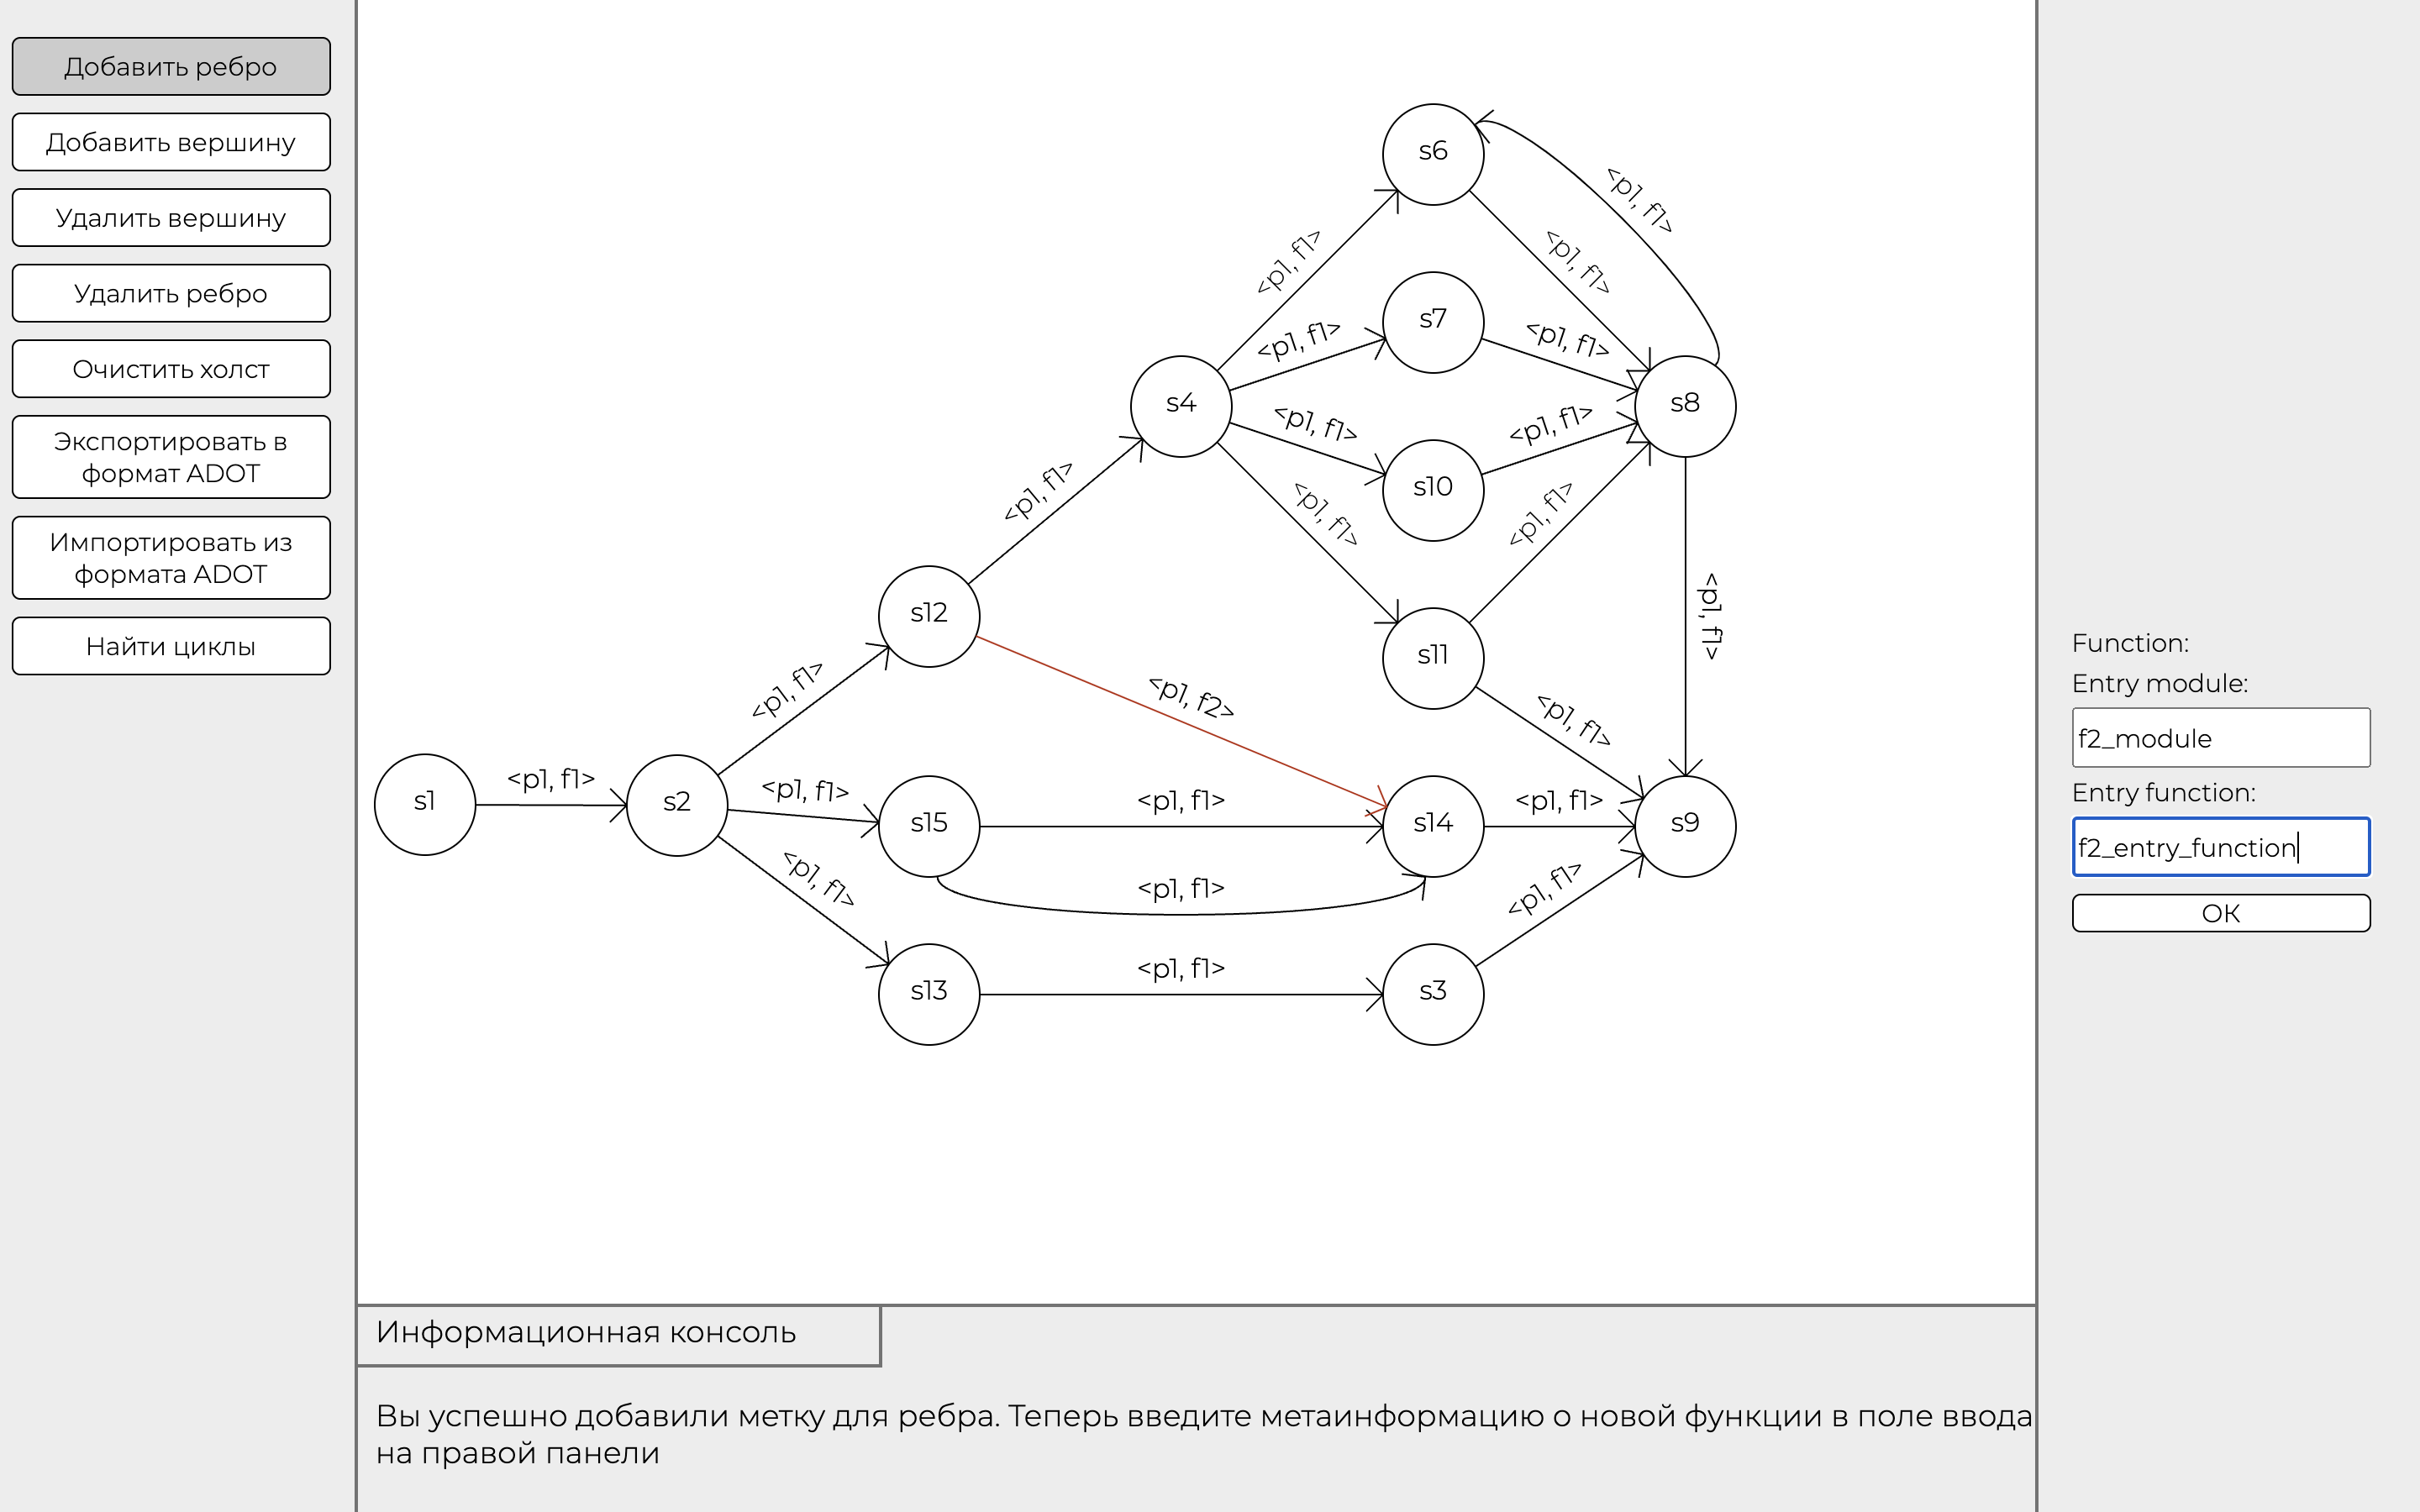
\includegraphics[width=0.9\linewidth]{ResearchNotes/images/edge_create.png}}
\caption{Создание ребра}
\label{fig:edge_create}
\end{figure}

Дополнительный функционал сценария:
\begin{itemize}
	\item Блокировка создания ребра из вершины в нее же саму.
	\item Если между вершинами уже существуют ребра, то система построит ребро, используя кривые Безье.
	\item Если на момент построения ребра из вершины выходит только одно ребро, то система потребует учтонения типа параллелизма (формат aDOT).
	\item Если предикат или функция не являются уникальными в рамках графа, то не требуется уточнение информации о module и entry func.
\end{itemize}

Сложности при реализации сценария:
\begin{itemize}
	\item Использование множества вспомогательных функций: подсчет количества ребер между вершинами, для определения типа построения ребра (прямое или кривые Безье), подсчет количества ребер выходящих из вершины для уточнения типа параллелизма, проверка полей ввода предиката и функции (предикат может быть неопределен, а функция должна быть определена), проверка введенных предиката и функции на уникальность в рамках графа.
	\item Выбор типа построения ребра: прямое, кривые Безье. Обработка ситуации, когда пользователь создает цикл между этими вершинами.
\end{itemize}

Будущее расширение функционала сценария:
\begin{itemize}
	\item Возможность перевыбора вершин для построения ребра между ними. На данный момент нельзя допустить ошибку при выборе вершин, необходимо закончить процесс построения ребра, удалить его и создать новое, выбрав другие вершины.
	\item Алгоритм для построения ребра с использованием кривых Безье. На данный момент ребро строится с помощью одной кривой Безье, что не позволяет строить ребра более сложного вида, тем самым разрешая коллизии, когда ребро проходит через другие вершины.
\end{itemize}

\textbf{Удаление вершины}

Для удаления вершины необходимо выбрать соответствующий пункт в меню, а затем кликнуть на вершину для удаления - вершина удаляется с холста вместе со всеми связанными с ней ребрами.

Сложности при реализации сценария:
\begin{itemize}
	\item Корректно удалить все связанные с вершиной ребра, а затем удалить информацию об этих ребрах и связанных вершин.
\end{itemize}

Будущее расширение функционала сценария:
\begin{itemize}
	\item Возможность одновременного выбора нескольких вершин для удаления.
	\item Возможность откатить действия в том случае если была удалена лишняя вершина. В целом это касается всего приложения, на данный момент любое действие неотвратимо.
\end{itemize}

\textbf{Удаление ребра}

Для удаления ребра необходимо выбрать соответствующий пункт в меню, а затем клкинуть на ребро для удаления - ребро удаляется с холста.

Сложности при реализации сценария:
\begin{itemize}
	\item Удалить информацию о ребре из связанных этим ребром вершин.
\end{itemize}

Будущее расширение функционала сценария:
\begin{itemize}
	\item Более корректный выбор ребра, на данный момент надо кликать ровно на ребро поскольку для перехвата события клика используется event.target.closest
	\item Возможность одновременного выбора нескольких ребер для удаления
\end{itemize}

\textbf{Экспорт в формат aDOT}

Для экспорта в формат aDOT необходимо выбрать соответствующий пункт в меню, а затем поочередно выбрать две вершины, которые будут являться стартовой и конечной вершиной соответственно. Затем сформируется текстовый файл с описание графа в формате aDOT и автоматически начнется его загрузка.

\textbf{Импорт из формата aDOT}

Для импорта из формата aDOT необходимо выбрать соответствующий пункт в меню, а затем выбрать файл для импорта. Далее система сама построит граф, сохранив всю необходимую информацию.

Сложности при реализации сценария:
\begin{itemize}
	\item Разработка алгоритма визуализации
\end{itemize}

Будущее расширение функционала сценария:
\begin{itemize}
	\item Разработка более гибкого алгоритма визуализации, который сможет работать с более сложными графами.
\end{itemize}

















